\chapter{系统组成及功能说明}

\section{系统整体介绍}

\subsection{系统架构}

TriHaRiscv SoC采用CPU与NPU异构协同工作结构，系统架构如图\ref{fig:system-architecture}所示。
CPU执行控制程序和通用运算，NPU承担矩阵乘累加等计算任务。存储访问和外设配置通过不同的总线路径连接，
片上RAM、外部存储控制器和用户扩展接口构成系统的存储与输入输出部分。

\begin{center}
\begin{minipage}{\linewidth}
\centering
\captionsetup{type=figure,hypcap=false}
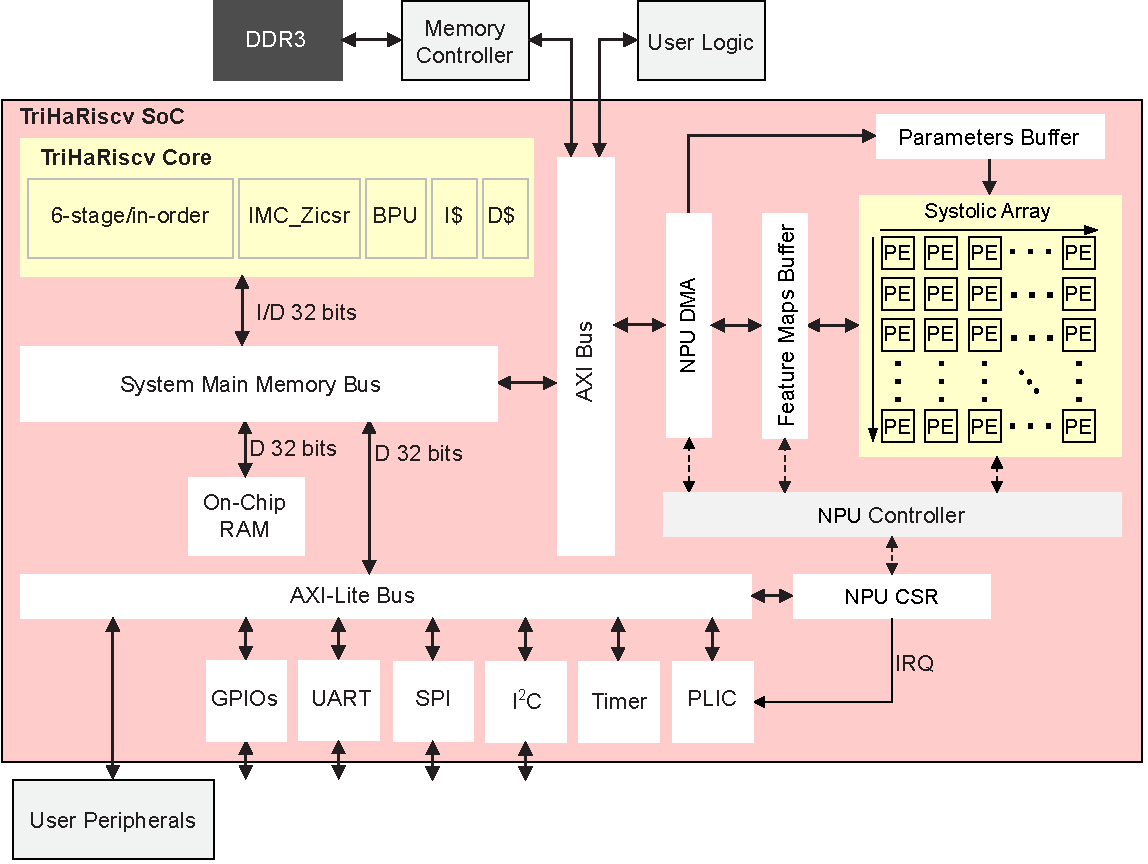
\includegraphics[width=\linewidth]{../figure/rv32-soc-page1.pdf}
\caption{TriHaRiscv SoC系统架构}\label{fig:system-architecture}
\end{minipage}
\end{center}

CPU采用六级双发射顺序执行结构，其指令和数据接口接入系统主存总线，连接片上RAM，
并经AXI通路访问外部存储。图中将DDR3及其存储控制器置于SoC边界之外，以区分处理
系统与板级存储接口。AXI-Lite通路用于访问外设寄存器和NPU控制寄存器，不承担NPU
的大批量数据搬运。

NPU包含控制器、DMA、特征图缓冲区、参数缓冲区和脉动阵列。CPU通过NPU控制寄存器
配置计算任务，DMA经AXI通路搬运特征图和参数，缓冲区为阵列提供计算数据。NPU控制
器协调数据传输和阵列运算，图中的中断通路用于返回任务完成通知。

SoC集成GPIO、UART、SPI、I\textsuperscript{2}C、定时器和PLIC等外设，各外设
通过AXI-Lite通路接入。PLIC汇聚NPU和外设的中断请求，并通知CPU处理。用户逻辑
和自定义外设分别通过相应的扩展接口接入系统。

\subsection{模块功能}

TriHaRiscv SoC划分为CPU、NPU、总线、存储、外设和视频六个模块，模块组成如图\ref{fig:soc-modules}所示。CPU和NPU分别封装为\texttt{triha\_cpu}和\texttt{triha\_npu}，其余模块提供系统互连、存储访问、外设控制及图像采集与显示功能。

\begin{center}
\begin{minipage}{\linewidth}
\centering
\captionsetup{type=figure,hypcap=false}
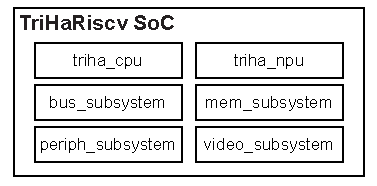
\includegraphics[width=0.5\linewidth]{../figure/rv32-soc-page2.pdf}
\caption{TriHaRiscv SoC模块图}\label{fig:soc-modules}
\end{minipage}
\end{center}

CPU通过\texttt{bus\_subsystem}访问存储空间和外设寄存器，并向NPU提交计算任务。
NPU通过DMA读取特征图和参数、写回计算结果；\texttt{mem\_subsystem}提供片上RAM
和外部存储的接入。\texttt{periph\_subsystem}集成通用外设及PLIC，将外设事件和
NPU任务完成中断送至CPU。

\texttt{video\_subsystem}完成像素接收、输入预处理、帧缓存管理和显示输出，CPU
负责视频链路配置、推理任务调度及显示结果发布。各模块的主要功能和接口见表\ref{tbl:module-roles}。

\begin{reporttable}
\begin{longtable}{@{}p{0.25\linewidth}p{0.41\linewidth}p{0.29\linewidth}@{}}
\caption{SoC模块功能表}\label{tbl:module-roles}\\
\toprule
模块 & 主要功能 & 主要接口 \\
\midrule
\endfirsthead
\caption[]{SoC模块功能表（续）}\\
\toprule
模块 & 主要功能 & 主要接口 \\
\midrule
\endhead
\bottomrule
\endfoot
\texttt{triha\_cpu} & 执行控制程序和通用运算，处理中断和异常 & 指令与数据访存接口、中断输入 \\
\texttt{triha\_npu} & 执行矩阵乘累加，调度DMA传输和阵列计算 & AXI数据接口、AXI-Lite寄存器接口、完成中断 \\
\texttt{bus\_subsystem} & 连接系统主从设备，完成地址译码、访问仲裁和协议桥接 & 主存总线、AXI与AXI-Lite接口 \\
\texttt{mem\_subsystem} & 提供片上RAM及外部存储接入，组织系统存储空间 & 片上RAM接口、外部存储访问接口 \\
\texttt{periph\_subsystem} & 集成GPIO、UART、SPI、I\textsuperscript{2}C、定时器和PLIC & AXI-Lite寄存器接口、外设信号与中断接口 \\
\texttt{video\_subsystem} & 完成图像采集、输入预处理、帧缓存管理和显示输出 & 视频输入输出接口、帧缓存读写接口 \\
\end{longtable}
\end{reporttable}

\section{CPU设计}

\subsection{CPU微架构}

{[}待填写{]}

\subsection{指令提取}

{[}待填写{]}

\subsection{指令译码}

{[}待填写{]}

\subsection{指令发射}

{[}待填写{]}

\subsection{指令执行}

{[}待填写{]}

\subsection{指令提交}

{[}待填写{]}

\subsection{存储管理}

{[}待填写{]}

\subsection{中断和异常}

{[}待填写{]}

\section{NPU设计}

\subsection{NPU微架构}

{[}待填写：总体框图、模块连接、支持的计算任务、CPU与NPU的协作关系，以及一次计算的执行流程。{]}

\subsection{PE计算单元}

{[}待填写：乘法器和累加器结构、输入与累加位宽、有符号运算、操作数传递，以及清零和使能控制。{]}

\subsection{脉动阵列}

{[}待填写：阵列规模、PE排列、边界接口、阵列互连、数据传播方向，以及结果读出方式。{]}

\subsection{阵列控制器}

{[}待填写：操作数锁存、波前注入、控制状态机、清零或续累加模式、计算时序、结束判定及完成握手。{]}

\subsection{DMA控制器}

{[}待填写：DDR数据搬入和结果写回、AXI突发传输、地址对齐、本地缓冲与预取、描述符队列、任务调度，以及背压和总线错误处理。{]}

\subsection{卷积展开单元}

{[}待填写：Im2Col实现、输入布局与寻址、卷积参数、边界补零、数据打包、硬件支持范围，以及功能关闭时的软件回退。{]}

\subsection{定点后处理单元}

{[}待填写：仿射变换、移位缩放、舍入规则、INT8饱和、零点与激活处理，以及硬件功能开关和软件分工。{]}

\subsection{寄存器接口}

{[}待填写：MMIO寄存器映射、字段定义、读写属性、软件配置和启动顺序、状态查询、状态清除，以及中断通知机制。{]}

\section{系统互连与存储}

\subsection{总线结构}

{[}待填写：控制总线和数据总线、主从设备连接、访问宽度，以及必要的协议桥接和跨时钟域路径。{]}

\subsection{存储组织}

{[}待填写：片上RAM和DDR的容量与组织、地址映射、缓存别名、模型参数和运行工作区分配、字节序，以及各区域的用途和访问限制。{]}

\begin{reporttable}
\begin{longtable}{@{}p{0.23\linewidth}p{0.34\linewidth}p{0.35\linewidth}@{}}
\caption{系统地址映射表}\\
\toprule
区域 & 实际地址 & 用途与访问限制 \\
\midrule
\endfirsthead
\caption[]{系统地址映射表（续）}\\
\toprule
区域 & 实际地址 & 用途与访问限制 \\
\midrule
\endhead
\bottomrule
\endfoot
{[}待填写{]} & {[}待填写{]} & {[}待填写{]} \\
{[}待填写{]} & {[}待填写{]} & {[}待填写{]} \\
{[}待填写{]} & {[}待填写{]} & {[}待填写{]} \\
{[}待填写{]} & {[}待填写{]} & {[}待填写{]} \\
\end{longtable}
\end{reporttable}

\subsection{访问仲裁}

{[}待填写：CPU、NPU和视频链路的并发请求、仲裁策略、事务归属、占用与释放条件，以及背压处理。{]}

\subsection{共享数据访问约定}

{[}待填写：缓存与DMA的数据可见性、共享缓冲区访问权限、数据同步顺序、缓存维护要求、软件维护责任，以及一致性约定。{]}

\section{图像采集与显示链路}

\subsection{图像采集}

{[}待填写：传感器初始化、DVP接口、像素接收、有效帧判据、输入像素格式、写入完整性，以及采集错误处理。{]}

\subsection{输入预处理}

{[}待填写：图像裁剪、像素格式转换、数据打包、模型输入生成，以及软硬件分工。{]}

\subsection{帧缓存管理}

{[}待填写：帧缓存容量和布局、帧标识、任务及模型标识、采集/推理/显示的缓冲区所有权转移、结果发布原子性、丢帧策略，以及复位和错误恢复。{]}

\subsection{显示输出}

{[}待填写：帧数据读取、扫描时序、原图与结果的同帧配对、显示接口配置，以及像素输出格式。{]}

\section{模型部署}

\subsection{模型选型}

{[}待填写：模型来源、许可证、网络结构、输入输出规格、输入尺寸和颜色顺序，以及选择依据。{]}

\subsection{量化方案}

{[}待填写：权重和激活的数据类型、量化参数、累加位宽、混合精度处理、舍入和溢出约定，以及数值参考。{]}

\subsection{模型导出}

{[}待填写：计算图描述、参数文件、张量布局、模型元数据、版本和哈希标识、部署文件生成方式，以及完整性检查。{]}

\subsection{算子映射}

{[}待填写：各算子及执行阶段的CPU/NPU分工、硬件支持范围、分块执行、软件回退条件，以及数值参考和限制。{]}

\begin{reporttable}
\begin{longtable}{@{}p{0.18\linewidth}p{0.24\linewidth}p{0.22\linewidth}p{0.30\linewidth}@{}}
\caption{算子执行方式表}\\
\toprule
算子或阶段 & 执行后端 & 实际支持范围 & 数值参考与限制 \\
\midrule
\endfirsthead
\caption[]{算子执行方式表（续）}\\
\toprule
算子或阶段 & 执行后端 & 实际支持范围 & 数值参考与限制 \\
\midrule
\endhead
\bottomrule
\endfoot
{[}待填写{]} & {[}待填写{]} & {[}待填写{]} & {[}待填写{]} \\
{[}待填写{]} & {[}待填写{]} & {[}待填写{]} & {[}待填写{]} \\
{[}待填写{]} & {[}待填写{]} & {[}待填写{]} & {[}待填写{]} \\
{[}待填写{]} & {[}待填写{]} & {[}待填写{]} & {[}待填写{]} \\
\end{longtable}
\end{reporttable}

\subsection{裸机运行时}

{[}待填写：软件层次、启动初始化、链接布局、模型加载、MMIO驱动调用、固定工作区、张量缓冲复用、资源生命周期、日志和错误返回。{]}

\subsection{推理流程}

{[}待填写：软件入口、输入准备、调用链、逐层调度、任务提交和完成检查、后处理、结果交付、失败回退，以及输入输出接口。{]}

\section{FPGA实现}

FPGA顶层集成了SoC、时钟复位模块，以及存储和板级接口封装，模块组成如图\ref{fig:fpga-top-modules}所示。\texttt{triha\_soc}封装图\ref{fig:soc-modules}中的六个SoC模块，顶层通过各接口封装连接外部存储、摄像头、显示设备和通用外设。

\begin{center}
\begin{minipage}{\linewidth}
\centering
\captionsetup{type=figure,hypcap=false}
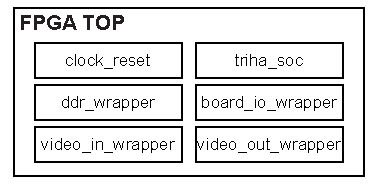
\includegraphics[width=0.5\linewidth]{../figure/rv32-soc-page3.pdf}
\caption{FPGA顶层模块图}\label{fig:fpga-top-modules}
\end{minipage}
\end{center}

\texttt{clock\_reset}根据板级参考时钟生成各时钟域的工作时钟，并按初始化顺序生成与释放复位信号。\texttt{ddr\_wrapper}封装DDR3控制器和厂商存储接口，为CPU、NPU及视频帧缓存提供外部存储访问通路。\texttt{board\_io\_wrapper}连接UART、GPIO、SPI和I\textsuperscript{2}C等板级信号，完成SoC内部接口与FPGA引脚之间的适配。

\texttt{video\_in\_wrapper}接入摄像头像素及帧、行同步信号，将其送入SoC视频子系统；\texttt{video\_out\_wrapper}接收视频子系统输出的像素和同步信号，连接板级显示接口。厂商IP及板级信号适配集中在顶层封装模块中，SoC内部保留处理、互连和视频链路的功能逻辑。

\subsection{目标平台}

本设计采用盘古100pro+开发板作为验证平台，主控为紫光同创Logos-2系列FPGA，器件型号为 PG2L100H-6IFBG676。CPU、NPU、系统互连和视频处理逻辑部署在该器件中，利用片上逻辑、APM运算单元和DRM存储块完成计算与数据缓冲。
板载DDR3由两颗4Gbit芯片组成，总容量为1GB，通过32bit数据通路连接FPGA，用于存放模型参数、特征图和视频帧。HDMI输入输出接口连接视频链路，USB-UART接口承担裸机程序的串口通信和调试。平台主要配置见表\ref{tbl:platform}。

\begin{reporttable}
\footnotesize
\begin{longtable}{@{}lll@{}}
\caption{平台配置表}\label{tbl:platform}\\
\toprule
项目 & 配置 & 说明或用途 \\
\midrule
\endfirsthead
\caption[]{平台配置表（续）}\\
\toprule
项目 & 配置 & 说明或用途 \\
\midrule
\endhead
\bottomrule
\endfoot
开发板 & 盘古100pro+（MES2L676-100HP） & FPGA及板级外设平台 \\
主控器件 & PG2L100H-6IFBG676 & 紫光同创Logos-2系列FPGA \\
逻辑资源 & 66,600个LUT，133,200个FF & CPU、NPU及系统控制逻辑 \\
运算资源 & 240个APM & 乘法与MAC运算 \\
片上存储 & 155个36Kbit DRM & CPU存储、Cache及NPU缓冲区 \\
外部存储 & 1GB DDR3，2颗4Gbit芯片，32bit数据位宽 & 模型参数、特征图及视频帧存储 \\
视频接口 & 1路HDMI输入、1路HDMI输出 & 视频接入与显示 \\
通信接口 & USB-UART & 板载通信与串口调试 \\
辅助接口 & 按键、LED、SD卡接口 & 控制输入、状态显示及扩展存储 \\
下载与供电 & JTAG、12V电源接口 & 比特流下载、逻辑调试和板卡供电 \\
\end{longtable}
\end{reporttable}

\subsection{工程配置}

{[}待填写：工具版本、顶层模块、源码组织、功能开关、厂商IP和官方例程的引用版本及修改范围，以及综合、布局布线和位流生成流程。{]}

\subsection{时钟复位}

{[}待填写：时钟来源、频率与PLL配置、时钟域划分、复位顺序、DDR初始化依赖以及跨域处理的总体安排。{]}

\subsection{板级接口}

{[}待填写：摄像头、显示、DDR和UART等板级接口的引脚映射、信号方向、I/O标准、电平要求、连接关系及接口配置。{]}

\subsection{实现约束}

{[}待填写：时钟约束、输入输出时序约束、跨域约束、时序例外及其依据、尚未确认的外部接口条件，以及约束覆盖范围和待闭合事项。{]}
